\documentclass[tikz,border=3mm]{standalone}
\usepackage{booktabs}
\usetikzlibrary{arrows.meta,backgrounds,positioning}

% This will generate multiple plots, one per page
% use `pdftk pdfname burst' to split into separate files
\begin{document}

\newcommand{\rankcontroller}{
  \foreach \x in {0, 1, 2, 3, 4} {
      \pgfmathsetmacro{\xx}{\x + 1}
      \node at (\xx, 0.5) {$R\x$};
      \draw[dotted] (\xx, 0) -- (\xx, -7);
    }

  \foreach \y in {1, 2, 3, 4, 5, 6} {
      \draw[dotted,thick] (-1,-\y) -- (6,-\y);
      \node[anchor=south east,text=black!40] at (-1, -\y) {T\y};
    }

  \begin{scope}[shift={(-0.0, 0)}]
    \draw[->,thick,-stealth] (0, 0) -- (0, -7)
    node[midway,sloped,above,rotate=180,fill=white,fill opacity=0.7] {Time};
  \end{scope}
}

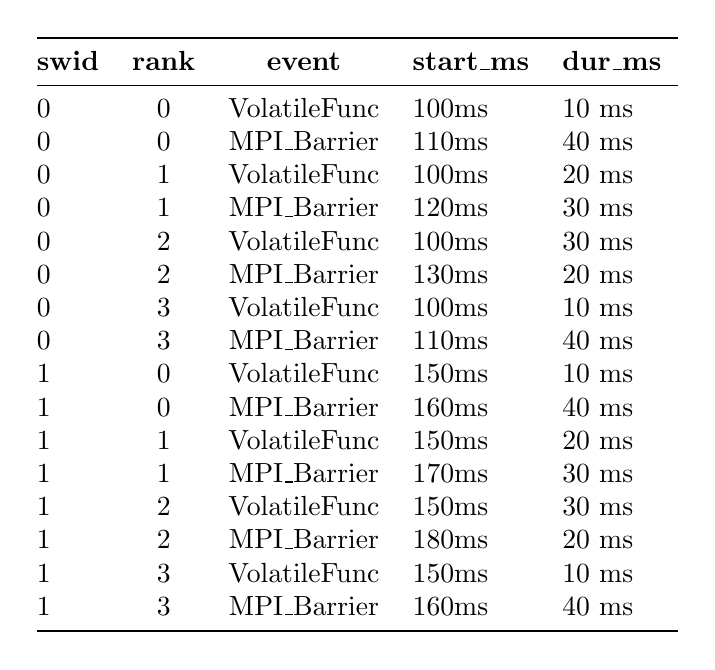
\begin{tikzpicture}

  \node[anchor=north west] at (0, 0) {
    \begin{tabular}
      {@{}lccllr@{}}
      \toprule
      \textbf{swid} & \textbf{rank} & \textbf{event} & \textbf{start\_ms} & \textbf{dur\_ms} \\
      \midrule
      0             & 0             & VolatileFunc   & 100ms              & 10 ms            \\
      0             & 0             & MPI\_Barrier   & 110ms              & 40 ms            \\
      0             & 1             & VolatileFunc   & 100ms              & 20 ms            \\
      0             & 1             & MPI\_Barrier   & 120ms              & 30 ms            \\
      0             & 2             & VolatileFunc   & 100ms              & 30 ms            \\
      0             & 2             & MPI\_Barrier   & 130ms              & 20 ms            \\
      0             & 3             & VolatileFunc   & 100ms              & 10 ms            \\
      0             & 3             & MPI\_Barrier   & 110ms              & 40 ms            \\
      1             & 0             & VolatileFunc   & 150ms              & 10 ms            \\
      1             & 0             & MPI\_Barrier   & 160ms              & 40 ms            \\
      1             & 1             & VolatileFunc   & 150ms              & 20 ms            \\
      1             & 1             & MPI\_Barrier   & 170ms              & 30 ms            \\
      1             & 2             & VolatileFunc   & 150ms              & 30 ms            \\
      1             & 2             & MPI\_Barrier   & 180ms              & 20 ms            \\
      1             & 3             & VolatileFunc   & 150ms              & 10 ms            \\
      1             & 3             & MPI\_Barrier   & 160ms              & 40 ms            \\
      \bottomrule
    \end{tabular}
  };

\end{tikzpicture}

\begin{tikzpicture}[
    rankbox/.style={rectangle, draw, minimum width=1.5cm, minimum height=0.8cm, fill=gray!20},
    thread/.style={dotted, thick},
    font=\Large
  ] % temporary, to visualize grid
  \node[font={\LARGE\bfseries}] at (3, 1.5) {BSP Trace};
  \rankcontroller
\end{tikzpicture}

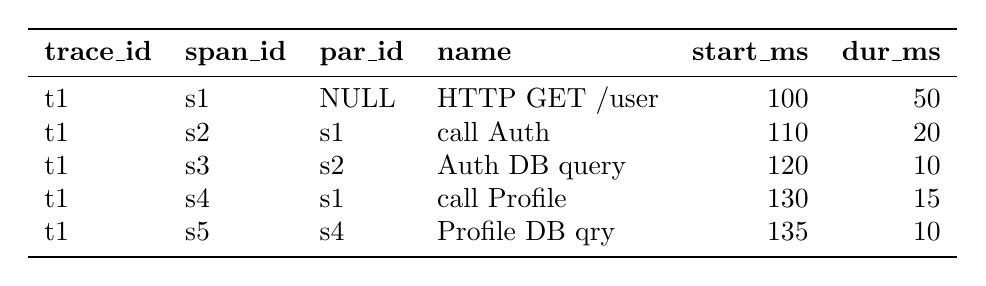
\begin{tikzpicture}
  \node[inner sep=0] (T) {
    \begin{tabular}{l l l l r r}
      \toprule
      \textbf{trace\_id} & \textbf{span\_id} & \textbf{par\_id} & \textbf{name}  & \textbf{start\_ms} & \textbf{dur\_ms} \\
      \midrule
      t1                 & s1                & NULL             & HTTP GET /user & 100                & 50               \\
      t1                 & s2                & s1               & call Auth      & 110                & 20               \\
      t1                 & s3                & s2               & Auth DB query  & 120                & 10               \\
      t1                 & s4                & s1               & call Profile   & 130                & 15               \\
      t1                 & s5                & s4               & Profile DB qry & 135                & 10               \\
      \bottomrule
    \end{tabular}
  };
\end{tikzpicture}

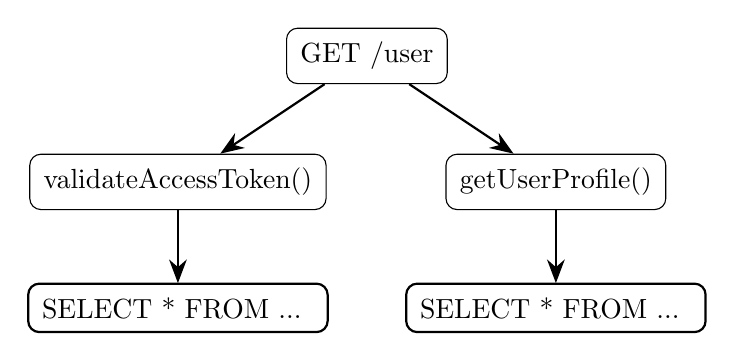
\begin{tikzpicture}
  [
  cgnode/.style={draw, rounded corners, align=center, inner sep=5pt, font=\normalsize},
  edge from parent/.style={draw,-{Stealth[length=3mm]}, line width=0.8pt},
  level distance=1.6cm,
  sibling distance=4.8cm
  ]
  \node[cgnode] (s1) {GET /user}
  child { node[cgnode] (s2) {validateAccessToken()}
      child { node[cgnode] (s3) {SELECT * FROM ... } }
    }
  child { node[cgnode] (s4) {getUserProfile()}
      child { node[cgnode] (s5) {SELECT * FROM ... } }
    };
\end{tikzpicture}

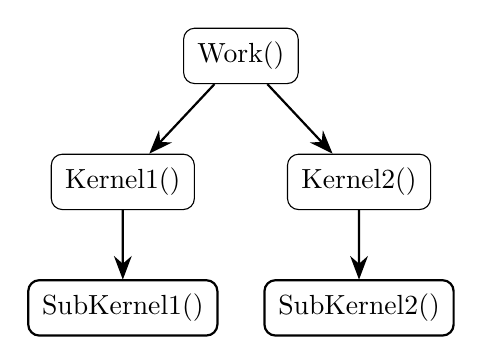
\begin{tikzpicture}
  [
  cgnode/.style={draw, rounded corners, align=center, inner sep=5pt, font=\normalsize},
  edge from parent/.style={draw,-{Stealth[length=3mm]}, line width=0.8pt},
  level distance=1.6cm,
  sibling distance=3.cm
  ]
  \node[cgnode] (s1) {Work()}
  child { node[cgnode] (s2) {Kernel1()}
      child { node[cgnode] (s3) {SubKernel1()} }
    }
  child { node[cgnode] (s4) {Kernel2()}
      child { node[cgnode] (s5) {SubKernel2()} }
    };
\end{tikzpicture}

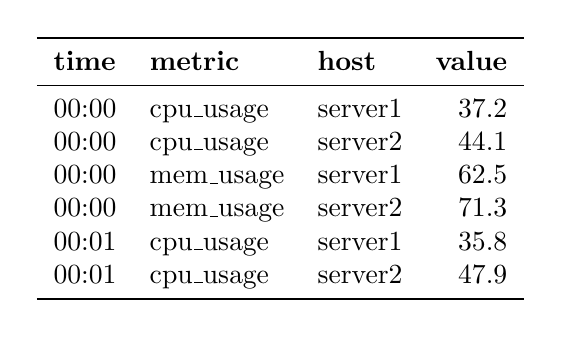
\begin{tikzpicture}
  \node[anchor=north west] at (0, 0) {
    \begin{tabular}{l l l r}
      \toprule
      \textbf{time} & \textbf{metric} & \textbf{host} & \textbf{value} \\
      \midrule
      00:00         & cpu\_usage      & server1       & 37.2           \\
      00:00         & cpu\_usage      & server2       & 44.1           \\
      00:00         & mem\_usage      & server1       & 62.5           \\
      00:00         & mem\_usage      & server2       & 71.3           \\
      00:01         & cpu\_usage      & server1       & 35.8           \\
      00:01         & cpu\_usage      & server2       & 47.9           \\
      \bottomrule
    \end{tabular}
  };
\end{tikzpicture}

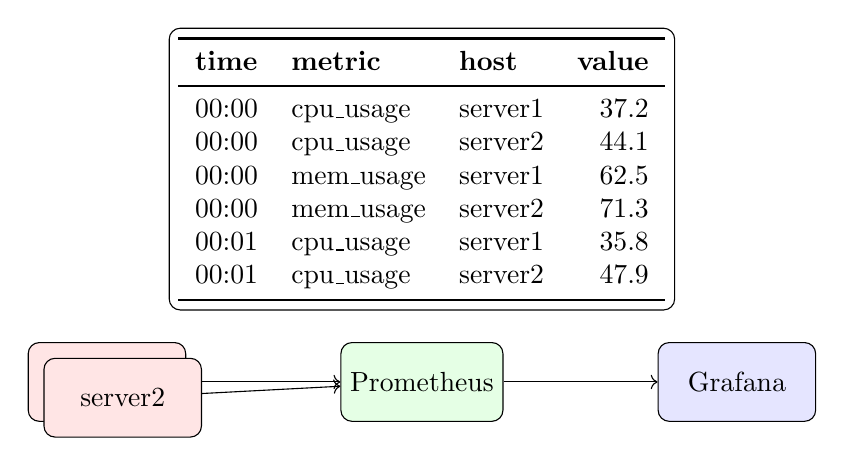
\begin{tikzpicture}[
    every node/.style={rectangle, rounded corners, draw, minimum width=2cm, minimum height=1cm}
  ]
  \node [fill=red!10] (s1) {server1};
  \node [fill=red!10] (s2) at ([xshift=2mm,yshift=-2mm]s1) {server2};
  \node [fill=green!10, right of=s1, node distance=4cm] (p) {Prometheus};
  \node [right of=p, node distance=4cm, fill=blue!10] (g) {Grafana};

  \begin{scope}[on background layer]
    \draw [->] (s1) -- (p);
    \draw [->] (s2) -- (p);
    \draw [->] (p) -- (g);
  \end{scope}

  \node[anchor=south,yshift=4mm] at (p.north) {
    \begin{tabular}{l l l r}
      \toprule
      \textbf{time} & \textbf{metric} & \textbf{host} & \textbf{value} \\
      \midrule
      00:00         & cpu\_usage      & server1       & 37.2           \\
      00:00         & cpu\_usage      & server2       & 44.1           \\
      00:00         & mem\_usage      & server1       & 62.5           \\
      00:00         & mem\_usage      & server2       & 71.3           \\
      00:01         & cpu\_usage      & server1       & 35.8           \\
      00:01         & cpu\_usage      & server2       & 47.9           \\
      \bottomrule
    \end{tabular}
  };

\end{tikzpicture}

\end{document}